\hypertarget{a00007}{
\section{crf::crfStarter Class Reference}
\label{a00007}\index{crf::crfStarter@{crf::crfStarter}}
}
This class provides easly handable \hyperlink{a00007_bff219a07f93750e4e6db09fd026de7f}{run()} methods to start an equalizer application with OSG scene data.  


{\tt \#include $<$crfStarter.h$>$}

Collaboration diagram for crf::crfStarter:\nopagebreak
\begin{figure}[H]
\begin{center}
\leavevmode
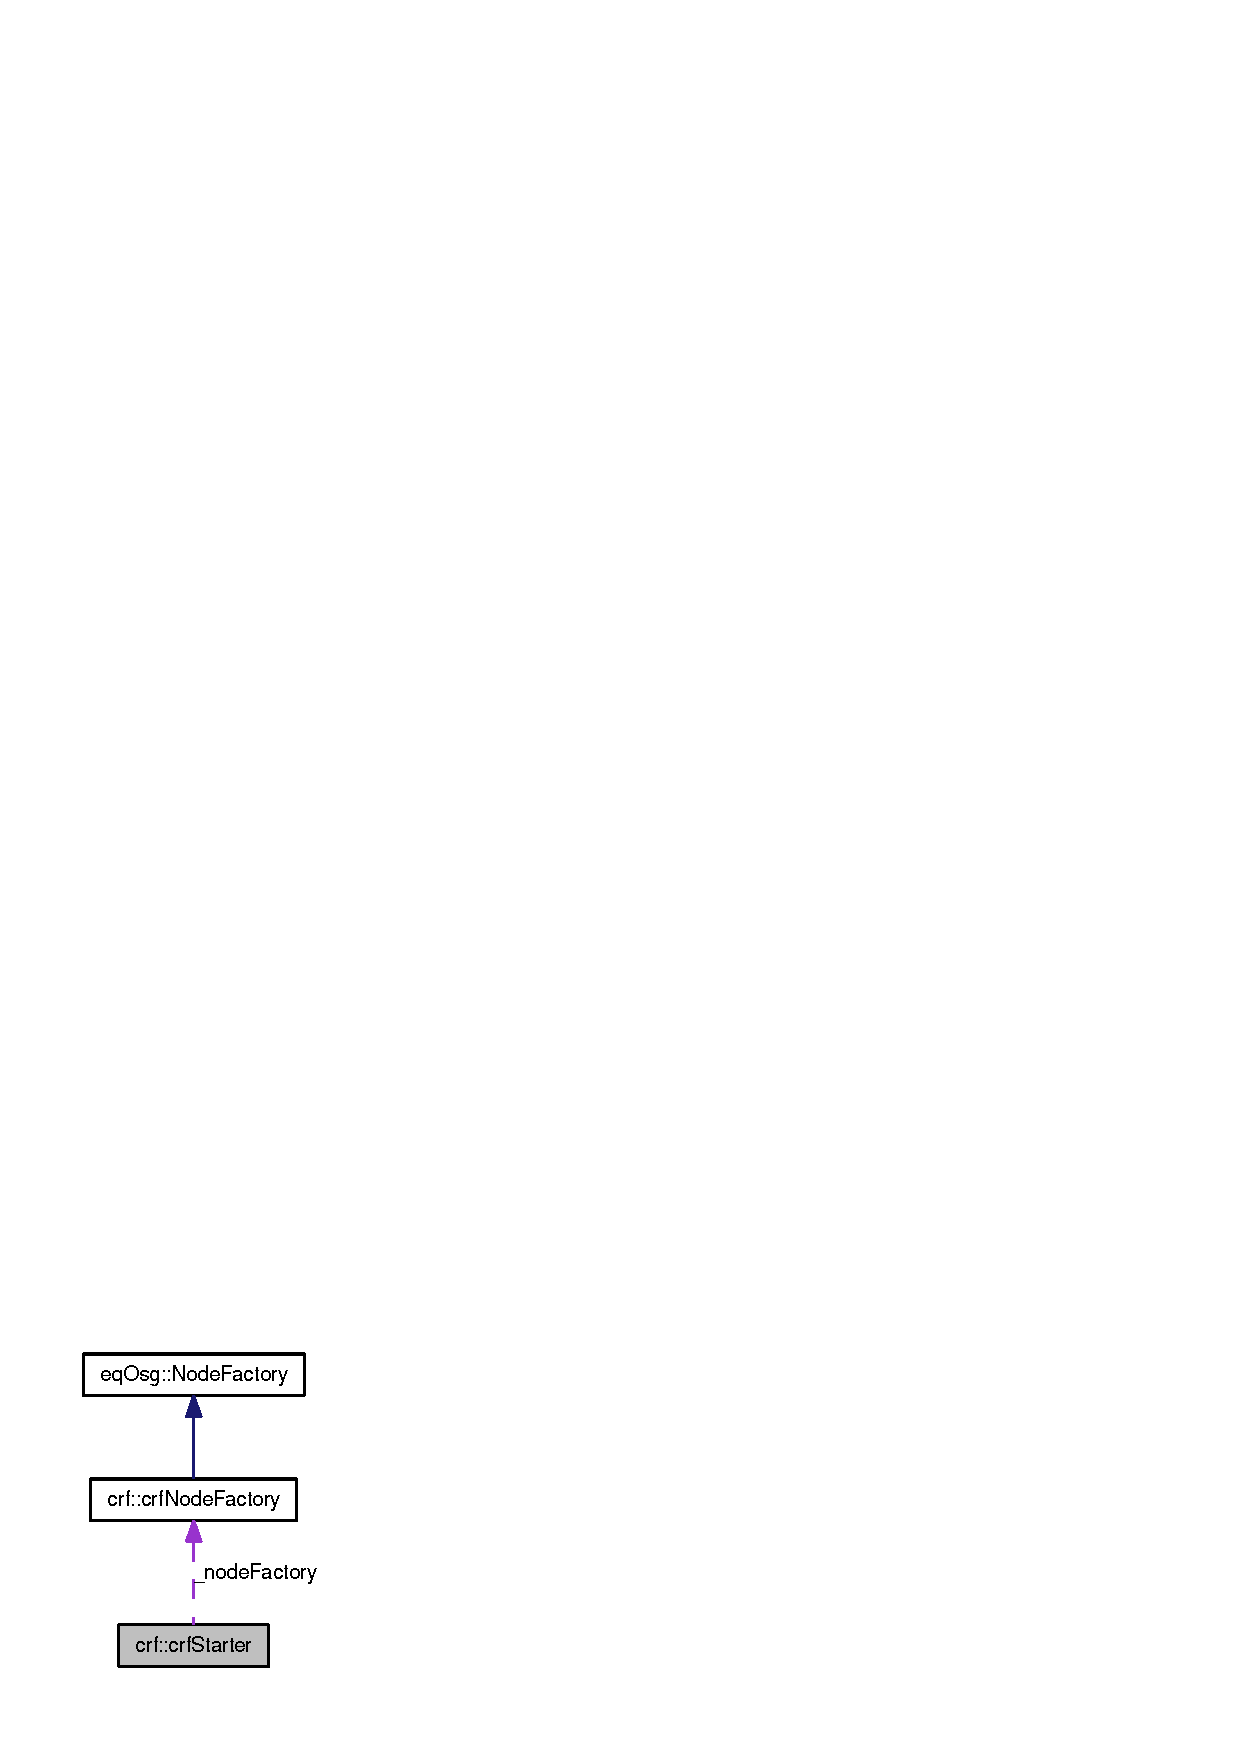
\includegraphics[width=156pt]{a00079}
\end{center}
\end{figure}
\subsection*{Public Member Functions}
\begin{CompactItemize}
\item 
\hypertarget{a00007_e1d24d865b4c98f43163acafc3a48fce}{
\hyperlink{a00007_e1d24d865b4c98f43163acafc3a48fce}{crfStarter} ()}
\label{a00007_e1d24d865b4c98f43163acafc3a48fce}

\begin{CompactList}\small\item\em Default constructor. Sets the viewer- and nodefactorypointer to zero. \item\end{CompactList}\item 
virtual int \hyperlink{a00007_bff219a07f93750e4e6db09fd026de7f}{run} (int argc, char $\ast$$\ast$argv)
\begin{CompactList}\small\item\em Initialize with arguments. \item\end{CompactList}\item 
virtual int \hyperlink{a00007_20c31de1c50c6504a4aaa617d606715b}{run} (int argc, char $\ast$$\ast$argv, osg::ref\_\-ptr$<$ osg::Node $>$ node)
\begin{CompactList}\small\item\em Initialises with arguments and the osg-node which should be displayed with equalizer. \item\end{CompactList}\item 
void \hyperlink{a00007_317832b54784e7c2c21f5d6bda17cda3}{setNodeFactory} (\hyperlink{a00005}{crfNodeFactory} $\ast$fac)
\begin{CompactList}\small\item\em Sets the custom node factory to provide the overriden \hyperlink{a00043}{crf} classes. \item\end{CompactList}\item 
std::string \hyperlink{a00007_b74ff2cc944f29fb91262ab5a9fa084a}{parseCommandLineForString} (int argc, char $\ast$$\ast$argv, std::string prefix)
\begin{CompactList}\small\item\em returns a string minus the passed prefix, if the prefix could be found \item\end{CompactList}\item 
\hyperlink{a00005}{crf::crfNodeFactory} $\ast$ \hyperlink{a00007_6b14742d2d820eba786626ab044c7cbd}{getNodeFactory} ()
\begin{CompactList}\small\item\em Gets the custom node factory. \item\end{CompactList}\end{CompactItemize}


\subsection{Detailed Description}
This class provides easly handable \hyperlink{a00007_bff219a07f93750e4e6db09fd026de7f}{run()} methods to start an equalizer application with OSG scene data. 

Actually these modes are supported: \begin{itemize}
\item Pass an osg::node as 3rd argument. This node will be the scene graph's root node \item Override \hyperlink{a00006}{crfPipe} and other \hyperlink{a00043}{crf} classes to create your more specific scene. Create a \hyperlink{a00005}{crf::crfNodeFactory} which generates the overriden classes and pass it with \hyperlink{a00007_317832b54784e7c2c21f5d6bda17cda3}{crfStarter::setNodeFactory()} to this starter class. \item Do nothing: The \char`\"{}HelloWorld\char`\"{} scene will be rendered.\end{itemize}


\subsection{Member Function Documentation}
\hypertarget{a00007_6b14742d2d820eba786626ab044c7cbd}{
\index{crf::crfStarter@{crf::crfStarter}!getNodeFactory@{getNodeFactory}}
\index{getNodeFactory@{getNodeFactory}!crf::crfStarter@{crf::crfStarter}}
\subsubsection[{getNodeFactory}]{\setlength{\rightskip}{0pt plus 5cm}{\bf crf::crfNodeFactory}$\ast$ crf::crfStarter::getNodeFactory ()\hspace{0.3cm}{\tt  \mbox{[}inline\mbox{]}}}}
\label{a00007_6b14742d2d820eba786626ab044c7cbd}


Gets the custom node factory. 

\begin{Desc}
\item[Returns:]The starter's viewer factory. \end{Desc}
\hypertarget{a00007_b74ff2cc944f29fb91262ab5a9fa084a}{
\index{crf::crfStarter@{crf::crfStarter}!parseCommandLineForString@{parseCommandLineForString}}
\index{parseCommandLineForString@{parseCommandLineForString}!crf::crfStarter@{crf::crfStarter}}
\subsubsection[{parseCommandLineForString}]{\setlength{\rightskip}{0pt plus 5cm}std::string crf::crfStarter::parseCommandLineForString (int {\em argc}, \/  char $\ast$$\ast$ {\em argv}, \/  std::string {\em prefix})}}
\label{a00007_b74ff2cc944f29fb91262ab5a9fa084a}


returns a string minus the passed prefix, if the prefix could be found 

\begin{Desc}
\item[Parameters:]
\begin{description}
\item[{\em argc}]argument counter \item[{\em argv}]command line arguments \item[{\em prefix}]the specified prefix \end{description}
\end{Desc}
\begin{Desc}
\item[Returns:]the to found string withou prefix \end{Desc}
\hypertarget{a00007_20c31de1c50c6504a4aaa617d606715b}{
\index{crf::crfStarter@{crf::crfStarter}!run@{run}}
\index{run@{run}!crf::crfStarter@{crf::crfStarter}}
\subsubsection[{run}]{\setlength{\rightskip}{0pt plus 5cm}virtual int crf::crfStarter::run (int {\em argc}, \/  char $\ast$$\ast$ {\em argv}, \/  osg::ref\_\-ptr$<$ osg::Node $>$ {\em node})\hspace{0.3cm}{\tt  \mbox{[}virtual\mbox{]}}}}
\label{a00007_20c31de1c50c6504a4aaa617d606715b}


Initialises with arguments and the osg-node which should be displayed with equalizer. 

\begin{Desc}
\item[Parameters:]
\begin{description}
\item[{\em argc}]CmdLine Argument Counter \item[{\em argv}]CmdLine Arguments \item[{\em node}]OSG Node \end{description}
\end{Desc}
\begin{Desc}
\item[Returns:]The cpp default main return value. \end{Desc}
\hypertarget{a00007_bff219a07f93750e4e6db09fd026de7f}{
\index{crf::crfStarter@{crf::crfStarter}!run@{run}}
\index{run@{run}!crf::crfStarter@{crf::crfStarter}}
\subsubsection[{run}]{\setlength{\rightskip}{0pt plus 5cm}int crf::crfStarter::run (int {\em argc}, \/  char $\ast$$\ast$ {\em argv})\hspace{0.3cm}{\tt  \mbox{[}virtual\mbox{]}}}}
\label{a00007_bff219a07f93750e4e6db09fd026de7f}


Initialize with arguments. 

\begin{Desc}
\item[Parameters:]
\begin{description}
\item[{\em argc}]CmdLine Argument Counter. \item[{\em argv}]CmdLine Arguments. \end{description}
\end{Desc}
\begin{Desc}
\item[Returns:]The cpp default main return value. \end{Desc}
\hypertarget{a00007_317832b54784e7c2c21f5d6bda17cda3}{
\index{crf::crfStarter@{crf::crfStarter}!setNodeFactory@{setNodeFactory}}
\index{setNodeFactory@{setNodeFactory}!crf::crfStarter@{crf::crfStarter}}
\subsubsection[{setNodeFactory}]{\setlength{\rightskip}{0pt plus 5cm}void crf::crfStarter::setNodeFactory ({\bf crfNodeFactory} $\ast$ {\em fac})\hspace{0.3cm}{\tt  \mbox{[}inline\mbox{]}}}}
\label{a00007_317832b54784e7c2c21f5d6bda17cda3}


Sets the custom node factory to provide the overriden \hyperlink{a00043}{crf} classes. 

\begin{Desc}
\item[Parameters:]
\begin{description}
\item[{\em fac}]The custom node factory. \end{description}
\end{Desc}


The documentation for this class was generated from the following files:\begin{CompactItemize}
\item 
E:/schule/Thesis/Repo/trunk/crf/src/crfStarter.h\item 
E:/schule/Thesis/Repo/trunk/crf/src/crfStarter.cpp\end{CompactItemize}
